\chapter{Lavori correlati}
\section{Long video understanding benchmarks}
La comprensione di video con una lunga durata richiede l'analisi e l'interpretazione di contenuti visivi che possono estendersi per diversi minuti o addirittura ore. Questi video richiedono metodi capaci di catturare sequenze temporali complesse e le interazioni tra più oggetti e persone, il che rende la loro gestione  particolarmente impegnativa dal punto di vista computazionale.

Per affrontare questa sfida sono stati sviluppati benchmark specifici che mettono alla prova la capacità dei modelli su questo tipo di task. Tra i più rilevanti troviamo EgoSchema \cite{mangalam2023egoschemadiagnosticbenchmarklongform}, un dataset con video egocentrici della durata massima di circa tre minuti, progettato per analizzare azioni quotidiane articolate in più passaggi. I video includono azioni semplici come manipolare strumenti e materiali di uso quotidiano. I modelli devono quindi avere una coerenza spaziotemporale dei vari movimenti, riconoscere pattern ricorrenti, e inferire correttamente le relazioni tra: mani, oggetti e azioni.

\begin{figure}[H]
    \centering
    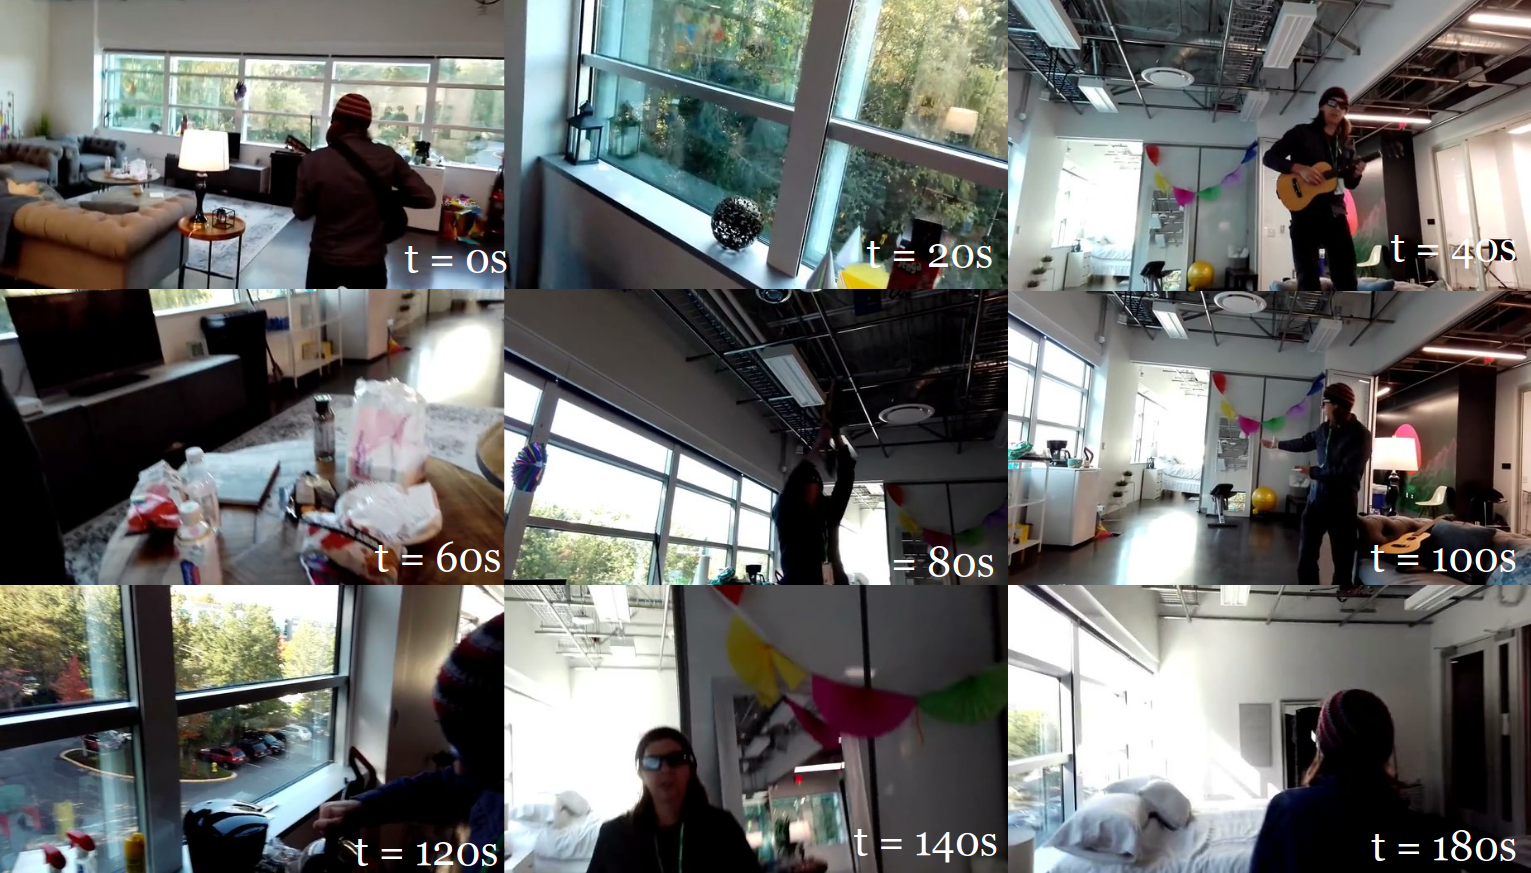
\includegraphics[width=0.65\textwidth]{Images/egoschema.png}
    \caption{EgoSchema Dataset}
    \label{fig:egoschema}
\end{figure}

ReST \cite{Yang_2023_CVPR} propone invece scenari industriali e scientifici più complessi, con video più lunghi in cui interagiscono simultaneamente più strumenti, oggetti e operatori.

Diversi approcci sono stati sviluppati: alcuni trattano il problema come un task di \emph{natural language question answering}, generando prima dei sottotitoli o descrizioni automatiche del video e utilizzando LLM per rispondere a domande specifiche \cite{ma2024drvideodocumentretrievalbased, park2025framesusefulefficientstrategies, wang2024videoagentlongformvideounderstanding, wang2024lifelongmemoryleveragingllmsanswering, wang2025videotreeadaptivetreebasedvideo, wu2022memvitmemoryaugmentedmultiscalevision}. Altri approcci integrano direttamente LLM con un encoder video, sfruttando le capacità di comprensione e generazione dei modelli linguistici per elaborare sequenze visive estese in maniera coerente \cite{li2024llmsmeetlongvideo, qian2024streaminglongvideounderstanding, ren2024timechattimesensitivemultimodallarge, song2024moviechatdensetokensparse}.

\section{Structured video representations}

Con \emph{rappresentazione strutturata} si intende l'insieme di tecniche volte a organizzare un video non come una semplice sequenza di frame, ma come una struttura semantica in grado di esplicitare le relazioni tra gli elementi presenti nella scena. Questo approccio consente di passare da una descrizione puramente visiva a una rappresentazione schematica e strutturata, che rende possibile interrogare i video in maniera più efficace, permettendo di estrarre informazioni mirate.

Un filone centrale della ricerca si è concentrato sullo studio delle relazioni contestuali, investigando in particolare i legami tra oggetti e attori \cite{arnab2021unifiedgraphstructuredmodels, baradel2018objectlevelvisualreasoning, cong2021spatialtemporaltransformerdynamicscene, jain2016structuralrnndeeplearningspatiotemporal, ji2019actiongenomeactionscomposition, ma2018attendinteracthigherorderobject, sun2018actorcentricrelationnetwork, wang2018videosspacetimeregiongraphs}. Parallelamente, sono stati proposti modelli basati su grafi per rappresentare le dipendenze tra azioni, al fine di catturare la dimensione temporale e causale dei comportamenti.

Lavori invece come UnweaveNet \cite{price2022unweavenetunweavingactivitystories} propogono di raggruppare i video in \emph{activity threads}, ossia insiemi di clip collegati logicamente che consentono di separare e ricostruire le diverse “storie” di attività intrecciate all'interno di una sequenza più lunga. Un altro contributo rilevante è l'introduzione dei cosiddetti \emph{egocentric scene graphs} \cite{rodin2023actionscenegraphslongform}, a cui hanno partecipato i professori Antonino Furnari e Giovanni Maria Farinella del Dipartimento di Matematica e Informatica dell'Università di Catania. Queste strutture sono progettate per rappresentare in modo esplicito le interazioni tra il soggetto che indossa la videocamera e gli oggetti presenti nell'ambiente.

\begin{figure}[H]
    \centering
    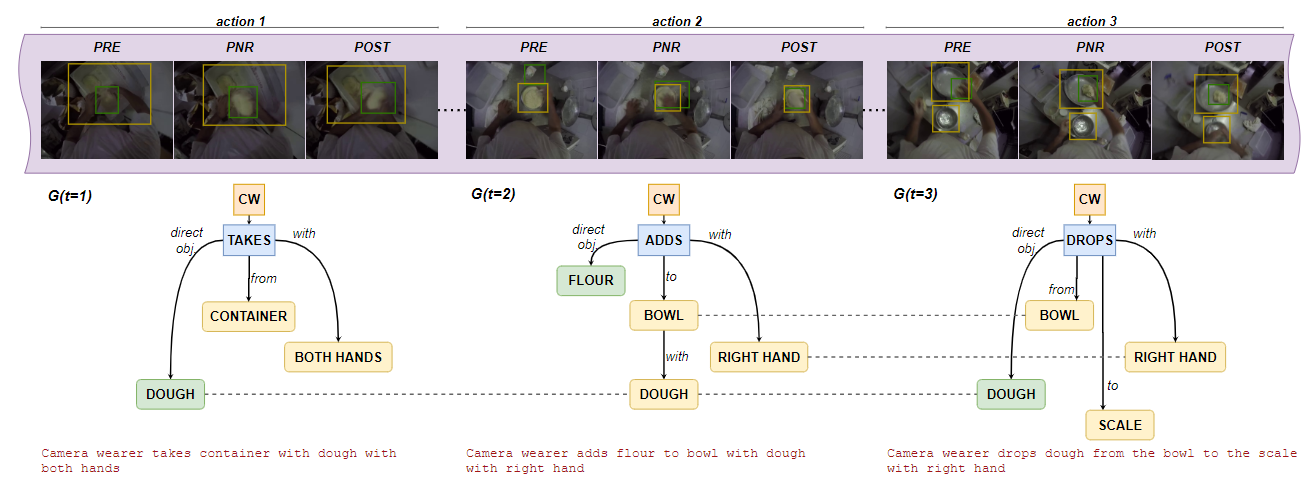
\includegraphics[width=0.7\textwidth]{Images/ego_graph.png}
    \caption{Egocentric scene graph. I nodi rappresentano attori e oggetti, mentre gli archi indicano le relazioni tra di essi.}
    \label{fig:ego_scene_graph}
\end{figure}

Nonostante questi progressi, tali approcci risultano ancora limitati, poiché tendono a catturare soltanto alcuni aspetti delle attività. In particolare, faticano a integrare in un unico modello le molteplici dimensioni tipiche dei video egocentrici: le interazioni con gli oggetti, i luoghi chiave in cui esse avvengono e le interdipendenze tra questi elementi. Questa mancanza di completezza riduce la capacità di ottenere rappresentazioni realmente efficaci.

\section{Video summarization}

Il riassunto del video ha come obiettivo la generazione di una versione ridotta di un video, tipicamente attraverso l'estrazione di \emph{key frames} che ne catturino i momenti salienti. Gli approcci proposti in letteratura variano in funzione degli elementi ritenuti rilevanti per la sintesi: alcuni si focalizzano sulla presenza e sul ruolo delle persone o degli oggetti all'interno della scena \cite{6247820}, altri privilegiano la rilevazione di eventi significativi \cite{Lu_2013_CVPR}, mentre ulteriori metodi considerano anche caratteristiche estetiche dei fotogrammi chiave per selezionare i contenuti più rappresentativi \cite{10.1007/978-3-319-10602-1_19}. 

Accanto a questi, sono stati introdotti approcci in grado di generare i riassunti in modalità \emph{online}, ossia durante la riproduzione del flusso video, consentendo una sintesi in tempo reale \cite{Lin_2015_ICCV_Workshops,Zhao_2014_CVPR}. Tuttavia, tali tecniche non costruiscono una rappresentazione strutturata del video e risultano spesso sensibili al rumore prodotto dai modelli di rilevamento, mancando di un'efficace integrazione della dimensione temporale.

Un contributo particolarmente rilevante in questa direzione è rappresentato da \cite{Xiong_2015_ICCV}, che permette di interrogare i contenuti lungo diverse dimensioni, anche combinandoli attraverso operatori booleani. Ciononostante, il metodo rimane in gran parte vincolato al riconoscimento di attrazioni predefinite e di oggetti visivamente distinti, risultando meno efficace in scenari affollati e caotici.